% !TEX encoding = UTF-8 Unicode
%!TEX TS-program = xelatex

\documentclass[12pt]{extarticle}
% extarticle is like article but can handle 8pt, 9pt, 10pt, 11pt, 12pt, 14pt, 17pt, and 20pt text

\def \ititle {Origins of Mind}
 
\def \isubtitle {Lecture 08}
 
\def \iauthor {Stephen A. Butterfill}
\def \iemail{s.butterfill@warwick.ac.uk}
\date{}

%for strikethrough
\usepackage[normalem]{ulem}

\usepackage{pdfpages}


\input{$HOME/Documents/submissions/preamble_steve_handout}

%logic symbol \leftmodels
\usepackage{MnSymbol}

%\bibpunct{}{}{,}{s}{}{,}  %use superscript TICS style bib
%remove hanging indent for TICS style bib
%TODO doesnt work
\setlength{\bibhang}{0em}
%\setlength{\bibsep}{0.5em}


%itemize bullet should be dash
\renewcommand{\labelitemi}{$-$}

\begin{document}

%\raggedcolumns

\begin{multicols*}{3}

\setlength\footnotesep{1em}


\bibliographystyle{newapa} %apalike

%\maketitle
%\tableofcontents




%--------------- 
%--- start paste

\def \ititle {Logic I}
 
\def \isubtitle {Lecture 11}
 
\begin{center}
 
{\Large
 
\textbf{\ititle}: \isubtitle
 
}
 
 
 
\iemail %
 
\end{center}
 
Readings refer to sections of the course textbook, \emph{Language, Proof and Logic}.
 
 
 
\section{Revision: ∀Elim, ∃Intro}
 
\emph{Reading:} §12.1, §13.1, §13.2
 
 
 
\section{∃Elim}
 
\emph{Reading:} §12.2, §13.2
 
\begin{center}
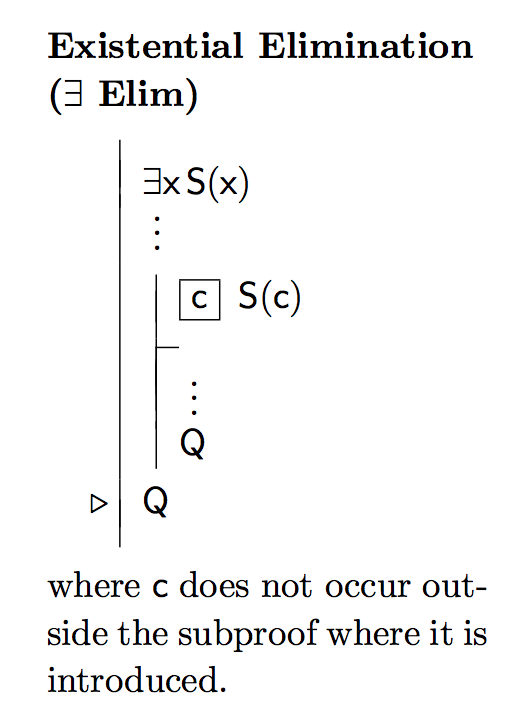
\includegraphics[scale=0.3]{img/rule_existential_elim.png}
\end{center}
\begin{center}
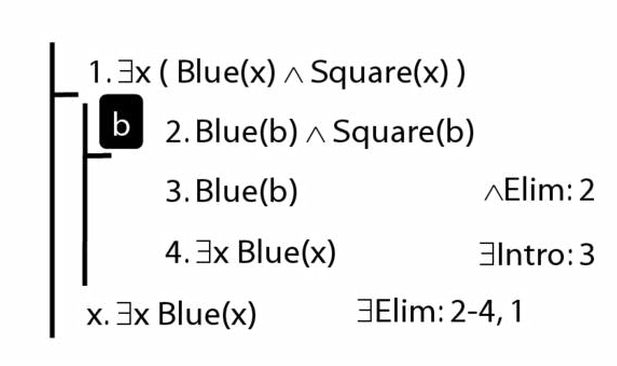
\includegraphics[scale=0.3]{img/proof_existential_elim.png}
\end{center}
\begin{minipage}{\columnwidth}
 
Note this restriction on the use of ∃Elim:
 
\begin{center}
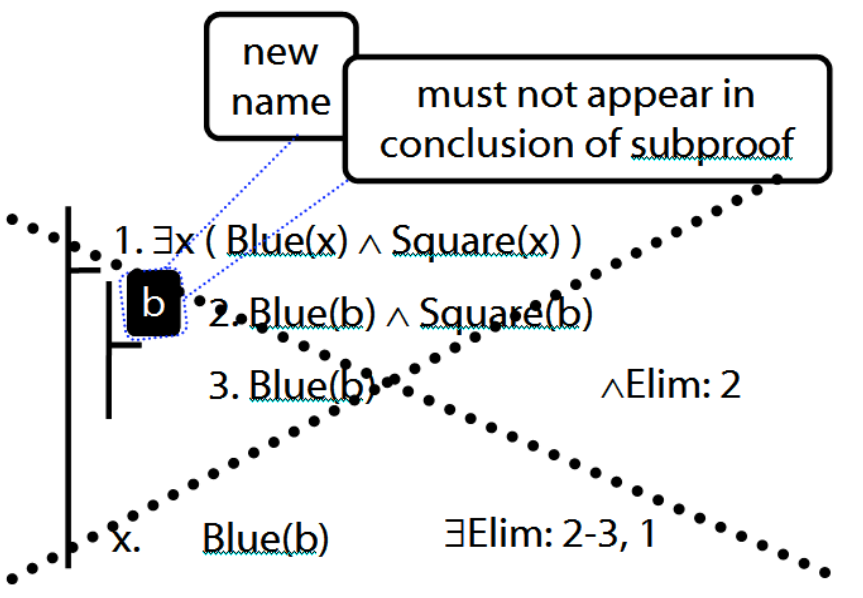
\includegraphics[scale=0.3]{img/proof_existential_elim_incorrect.png}
\end{center}
\end{minipage}
 
 
 
\section{Don't use ∃ with →}
 
\begin{minipage}{\columnwidth}
 
Is true ∃x(Square(x) → Broken(x)) in this world?
 
\begin{center}
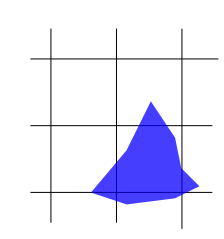
\includegraphics[scale=0.3]{img/word_02.png}
\end{center}
\end{minipage}
 
∃x(Square(x) → Broken(x))
 
\hspace{3mm} $\leftmodels\models$
 
∃x(¬Square(x) ∨ Broken(x))
 
\hspace{3mm} $\leftmodels\models$
 
∃x(¬Square(x)) ∨ ∃x(Broken(x))
 
 
 
\section{Watch Out, Here Come Multiple Quantifiers}
 
\emph{Reading:} §11.1
 
 
 
\section{Something Is Above Something}
 
\emph{Reading:} §11.1
 
\begin{minipage}{\columnwidth}
 
Something is above something:
 
\hspace{3mm} ∃x ∃y Above(x,y)
 
\end{minipage}
 
 
 \columnbreak
 
\section{Multiple Quantifiers: Everyone Likes Puffins}
 
\emph{Reading:} §11.1
 
I like puffins:
 
\hspace{3mm} ∀x ( Puffin(x) → Likes(a,x) )
 
y likes puffins:
 
\hspace{3mm} ∀x ( Puffin(x) → Likes(y,x) )
 
Everyone likes puffins:
 
\hspace{3mm} ∀y ∀x ( Puffin(x) → Likes(y,x) )
 
 
 
\section{Quantifiers Bind Variables}
 
\emph{Reading:} §9.3
 
\begin{center}
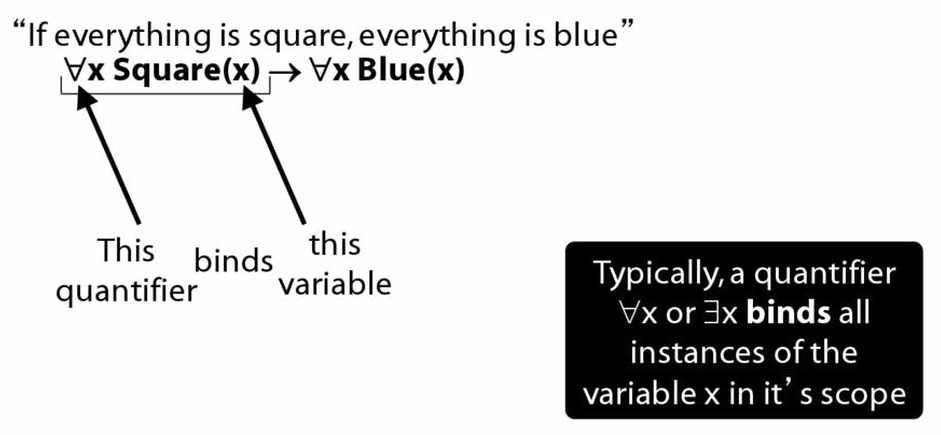
\includegraphics[scale=0.3]{img/quantifiers_scope.png}
\end{center}
 
 
\section{Summary of Quantifier Rules So Far}
 
\emph{Reading:} §12.1, §12.2, §12.3, §13.1, §13.2
 
 
 
\section{∀Intro}
 
\emph{Reading:} §12.1, §12.3, §13.1
 
\begin{center}
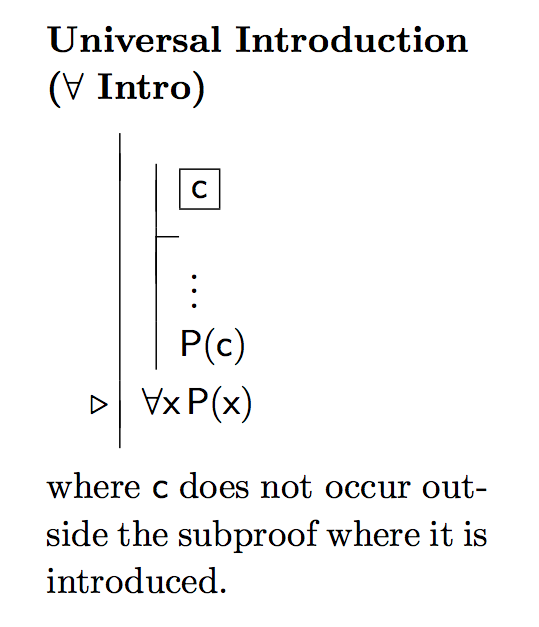
\includegraphics[scale=0.3]{img/rule_universal_intro.png}
\end{center}
\begin{center}
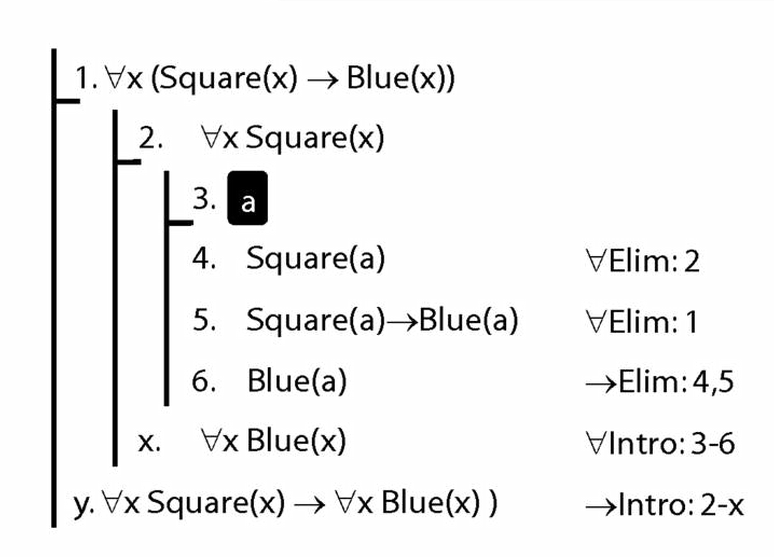
\includegraphics[scale=0.3]{img/proof_universal_intro.png}
\end{center}
\begin{minipage}{\columnwidth}
 
Why is this proof incorrect?
 
\begin{center}
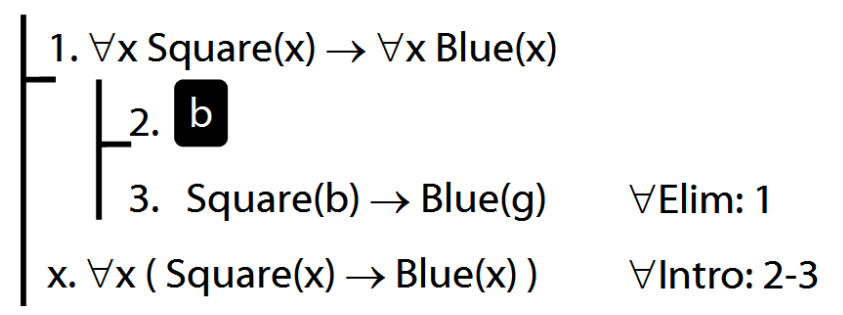
\includegraphics[scale=0.3]{img/proof_universal_intro_incorrect.png}
\end{center}
\end{minipage}
 
 
 
\section{∀Intro: An Incorrect Proof}
 
\emph{Reading:} §13.1, §13.2
 
This proof is wrong, but why?:
 
\begin{center}
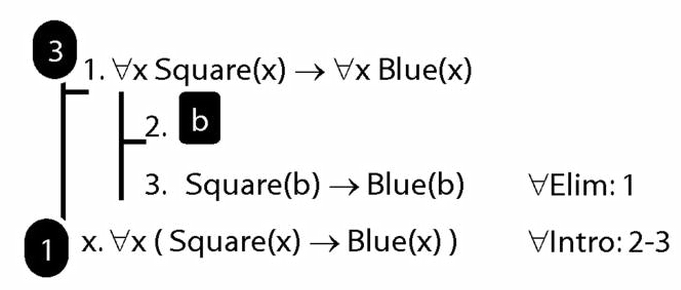
\includegraphics[scale=0.3]{img/unit_572_proof.png}
\end{center}
There is a counterexample to the argument:
 
\begin{center}
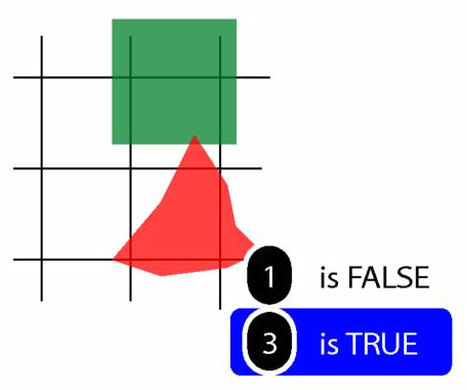
\includegraphics[scale=0.3]{img/unit_572_proof2.png}
\end{center}
\vfill
\begin{minipage}{\columnwidth}
\section{Exercises}
These exercises will be discussed in seminars the week after this lecture.
The numbers below refer to the numbered exercises in the course textbook, e.g.\ `1.1' refers to exercise 1.1. on page 39 of the second edition of \emph{Language, Proof and Logic}. Exercises marked `*' are optional.
 
\begin{quote}
6.17--6.20
 
6.33, 6.40
 
8.24--8.25
 
9.10
 
9.15--9.17
 
*9.18--9
 
11.2
 
12.4--12.5
 
*12.6--12.7
 
12.9--12.10
 
\end{quote}
\end{minipage}


%--- end paste
%--------------- 
 


\end{multicols*}

\end{document}